\documentclass[10pt]{article}
\usepackage[margin=0.8in]{geometry}
\usepackage[T1]{fontenc}
\usepackage[utf8]{inputenc}
\usepackage{lmodern,graphicx,booktabs,amsmath,amssymb,natbib,hyperref,float,placeins}
\hypersetup{colorlinks=true,linkcolor=blue,citecolor=blue,urlcolor=blue}
\graphicspath{{../../artifacts/coordination_injections/figures/}}
\setlength{\parskip}{4pt}
\setlength{\parindent}{0pt}
\renewcommand{\topfraction}{.9}
\renewcommand{\textfraction}{.08}
\renewcommand{\floatpagefraction}{.75}
\title{Verified adaptation of connected analytics artifacts after scoped user changes}
\author{OverseeingManyLLMs research package}
\date{12 September 2026}
\begin{document}
\maketitle
\begin{abstract}
We implement a protocol for adapting connected analytics artifacts after a scoped user change. It routes authorized corrections, executes proposed tools and checks actual uptake while preserving exceptions. A controlled study uses recorded UCI Online Retail transactions, sixteen constructed projects on eight monthly blocks, two generation replicas and fresh policy-specific GPU continuations. The frozen strict-parser study gives targeted delivery 31/32 complete structured projects in 100 calls, versus broadcast's 30/32 in 136. However, tool-envelope incompatibility confounds the larger apparent advantage over shared state. A separately declared exploratory follow-up accepts equivalent explicit envelopes and generates 250 fresh model responses in 80 continuations on inspected cases. Targeted and same-packet global checking each complete 16/16 projects in 46 calls, with identical request sequences. A deterministic pipeline completes all standardized contracts without model calls. The evidence supports scoped executable state management and exposes a parser confound, but does not establish a distinctive routing advance or reduced human workload. Generated prose can remain wrong despite correct numerical artifacts.
\end{abstract}

\section{Research question}
A person may revise a reporting requirement once while several agents hold old plans and outputs. The practical problem is to adapt connected work without extending the change into a protected exception. Agreement between agents is insufficient. A chart and report can agree with each other while using the wrong country, time period or metric.

We study a narrow operational protocol. A trusted application resolves an authorized change into scoped requirements. A controller routes correction packets, executes the agents' selected tools and checks whether affected artifacts actually changed. It expands delivery when targeted repair leaves invalid work. Our empirical question is whether this routing improves the correctness-cost tradeoff beyond a competent shared-state check and direct broadcast.

The study contributes an executable protocol with an explicit verification boundary, a controlled comparison on real transaction records, and an inspectable local demonstration. It does not introduce dependency invalidation, targeted prompting or multi-agent plan repair. A deterministic parameterized pipeline is included to test whether the application needs LLM agents at all.

\section{Protocol and verification boundary}
Four responsibilities form a registered graph: analysis $\rightarrow$ chart $\rightarrow$ report, with a separately scoped appendix. The analysis agent selects query parameters. A read-only SQL tool aggregates recorded transaction lines. The chart agent selects the parent table, displayed prefix and unit. The report agent selects the chart and unit; a tool supplies exact numerical claims. Generated prose remains available for inspection. The appendix retains the original reporting contract.

An instruction contains an authorized source, version, scope, exceptions and fields. An artifact records the consumed contract hash, its own revision, parent hashes, the model's tool proposal, executed evidence and unresolved issues. Peers can notify registered children and forward the immutable authorized packet. They cannot change its authority or scope. The local API validates the main-scope exception. This trust boundary assumes a trusted application and is not a network authentication mechanism.

After an update the controller inspects all artifacts. It calls selected roles in dependency order and checks each result. A second reconciliation round can expand to all remaining invalid roles. Each role receives at most two calls. An unchanged \texttt{keep} response preserves the old dependency hashes, so acknowledgment cannot certify uptake. A missing or failed artifact remains unfinished; dependent work cannot be released through an unaccepted parent.

The public guard checks query parameters against the applicable contract, executes SQL on a read-only snapshot and public sentinel rows, and checks chart and report dependencies. Independent evaluation aggregates the real rows in Python. Reference answers never enter packets or recipient selection. Finite sentinels alone do not establish universal SQL correctness. Tool compilation and arithmetic are supplied to every method and must receive credit for the correctness they enforce.

For four required artifacts, let $R$ count contract or numerical violations, $D$ count invalid/stale dependency checks, and $F$ count unfinished artifacts. We report each component and the authored diagnostic
\[
V = R/4 + \min(D,4)/4 + F/4, \qquad 0 \le V \le 3.
\]
The primary endpoint is complete correctness of the four \emph{structured} artifacts, alongside actual continuation calls. Unrestricted prose is not fully graded. Neither $V$ nor token counts are financial loss or measured mental workload.

The registered graph and two-round cap imply at most eight calls per continuation, or sixteen attempts with one retry per call. Main-scope changes preserve the appendix under the supported constructor and validated API. Acceptance requires current dependency hashes. These are software properties, not guarantees of semantic understanding or LLM compliance. We make no contraction or consensus-stability claim.

\section{Recorded data and constructed projects}
UCI Online Retail contains 541,909 recorded lines from one UK-based non-store retailer \citep{chen2015retail}. We preserve the complete source and audit it before choosing reporting conventions. The official archive is licensed CC BY 4.0. Its recorded dates run from 1 December 2010 to 9 December 2011. The final December is partial.

The audit finds 5,268 duplicate rows beyond the first, 135,080 missing customer IDs, 1,454 missing descriptions, 10,624 negative quantities and 1,336 negative-quantity rows without a cancellation prefix. There are 2,515 zero prices and two negative prices. These records remain in the raw snapshot. We do not infer profit, repair success or realized business losses.

Every query uses an inclusive start and exclusive end, retains duplicates, groups by stock code and orders totals descending with stock-code ties ascending. Positive non-cancellation lines require positive quantity and price and no cancellation prefix. Signed positive-price lines retain both quantity signs. The metric is either recorded quantity or recorded line value, $\sum q_i p_i$. Prices are represented exactly in millionths of GBP. These are declared reporting conventions, not claims that the source establishes an accounting definition of revenue.

Briefs, roles, changes, scopes and disturbances are authored. Changes affect country, period, missing-customer inclusion, positive versus signed lines, ranking metric or displayed prefix. Source transactions are real; the agent-team workload is constructed. The project endpoint is held fixed across methods, so adding roles cannot create additional utility.

\section{Design and implementation}
Development uses December 2010 and January 2011. Initial unrestricted SQL attempts frequently omitted required filters. A constrained query interface removed avoidable formatting and arithmetic burdens. Additional prompt repairs made explicit that a missing artifact should be created rather than blocked or kept. Every development request and interrupted attempt is retained. All four final development originals completed the four structured contracts before the evaluation freeze.

The primary matrix contains sixteen projects on eight disjoint monthly blocks, February through September 2011, with two generation replicas and four methods. Every method starts from the same pre-change checkpoint within a project/replica. Actual policy-specific GPU continuations are generated. Policy order rotates. The model is Qwen2.5-7B-Instruct at pinned revision \texttt{a09a354...8bc28}, BF16 on an RTX 6000 Ada, with temperature 0.3, top-$p$ 1, a 2,048-token context and 384 output tokens. Requests are serial, with no CPU offload.

\begin{description}
\item[Global shared state] Inspect every role and regenerate only invalid artifacts, with current resolved requirements and the shared project state.
\item[Active broadcast] Deliver the applicable packet to all four roles. Valid recipients may respond \texttt{keep}; processing the notification still uses a model call.
\item[Targeted injections] Send the same packet only to roles whose applicable contract changed, then expand if required.
\item[Sparse propagation] Initially send to affected roots. Generated notifications can reach registered children; a global fallback repairs missing propagation.
\end{description}
A matched-format control uses global invalidation with the same packets as targeted routing on replica 0 of all sixteen projects. A zero-inference pipeline directly selects tool parameters from the same contract. A separate matched stress condition corrupts a protected appendix parameter and value on the first project of each month, replica 0. A no-detailed-feedback ablation uses the same stress cases, current requirements and guards. Eight authored synthetic cases isolate propagation and failure boundaries.

The freeze precedes all evaluation generations. The primary cost comparison is targeted minus broadcast, with correctness reported alongside. Targeted versus global state is also declared. Two projects and both replicas are averaged inside each month before paired inference. We use 2,000 paired monthly-block bootstrap resamples with analysis seed 91843. There are eight blocks from one retailer, not sixteen independent organizations. Adjacent months can remain dependent. No noninferiority or equivalence margin is asserted.

\section{Results}
The 32 common originals all complete the four structured contracts. The frozen primary study gives the following results. Accepted numerical errors are zero for every method.
\begin{center}
\begin{tabular}{lrrrr}
\toprule
Method & Complete & Unfinished & Calls & Tokens \\
\midrule
Global state & 17/32 & 15 & 114 & 96,973 \\
Broadcast & 30/32 & 2 & 136 & 99,831 \\
Targeted & 31/32 & 1 & 100 & 75,985 \\
Sparse + fallback & 32/32 & 0 & 99 & 75,495 \\
Pipeline & 32/32 & 0 & 0 & 0 \\
\bottomrule
\end{tabular}
\end{center}
Targeted minus broadcast is -1.125 calls per project, with paired 95\% bootstrap interval [-1.3125, -1.0000]. Structured completion differs by +3.125 percentage points [0, 9.375], with one block win and seven ties. The large +43.75-point contrast with the original full shared-state presentation is parser-sensitive and cannot be attributed to recipient selection. Sixteen of eighteen unfinished leaf reports become locally valid when equivalent explicit tool envelopes are recognized. This diagnostic does not replace the saved trajectories.

The separately declared parser follow-up uses the same sixteen inspected projects at replica 0 and actual new continuations. It is exploratory, not a new held-out sample.
\begin{center}
\begin{tabular}{lrrrr}
\toprule
Method & Complete & Unfinished & Calls & Tokens \\
\midrule
Global state & 15/16 & 1 & 48 & 40,772 \\
Broadcast & 16/16 & 0 & 64 & 47,049 \\
Targeted & 16/16 & 0 & 46 & 35,187 \\
Sparse + fallback & 16/16 & 0 & 46 & 35,247 \\
Global, same packet & 16/16 & 0 & 46 & 35,187 \\
\bottomrule
\end{tabular}
\end{center}
Targeted and same-packet global checking have identical request sequences on all sixteen pairs. Their observed paired completion and call differences are zero in every block. The degenerate paired bootstrap interval [0,0] is not a population-equivalence claim. Active broadcast processes unaffected notifications and uses eighteen more calls. The remaining full-state failure uses an unsupported \texttt{parameters} envelope. No additional parser tuning or sample expansion follows.

\begin{figure}[!htbp]
\centering
\includegraphics[width=\linewidth]{quality_cost.pdf}
\caption{Original strict-parser study: real transaction data, constructed changes and GPU-generated tool choices. Quality is all four structured artifacts accepted and correct. Unfinished work is shown separately. Intervals resample eight monthly blocks; no human workload is measured.}
\end{figure}
\begin{figure}[!htbp]
\centering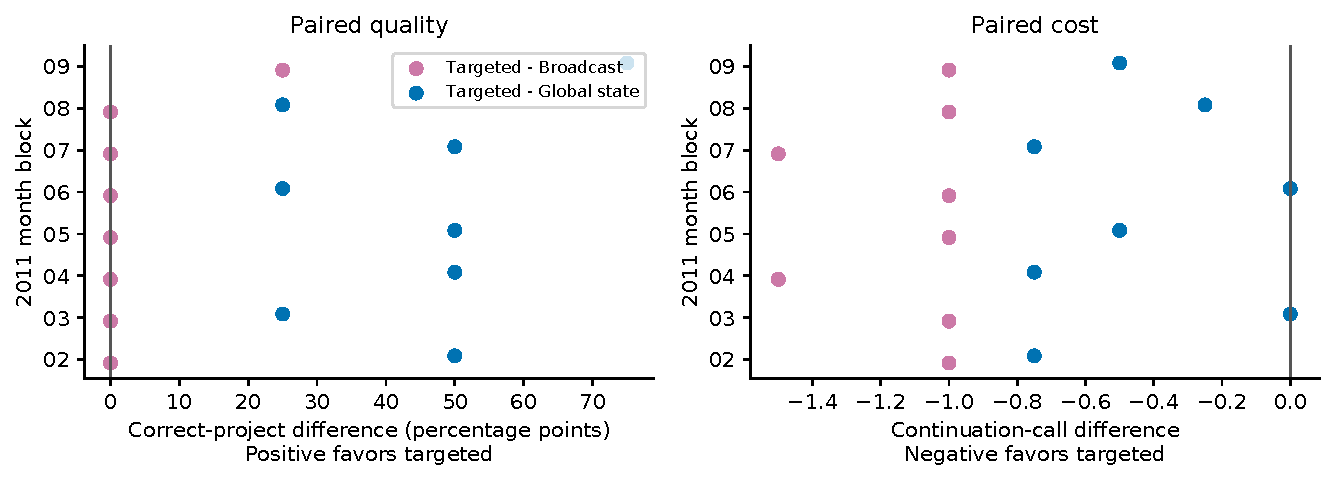
\includegraphics[width=\linewidth]{paired_blocks.pdf}
\caption{Paired monthly differences, averaging both projects and generation replicas. Positive correctness differences and negative call differences favor targeted routing. Ties and unfavorable blocks are retained.}
\end{figure}
\begin{figure}[!htbp]
\centering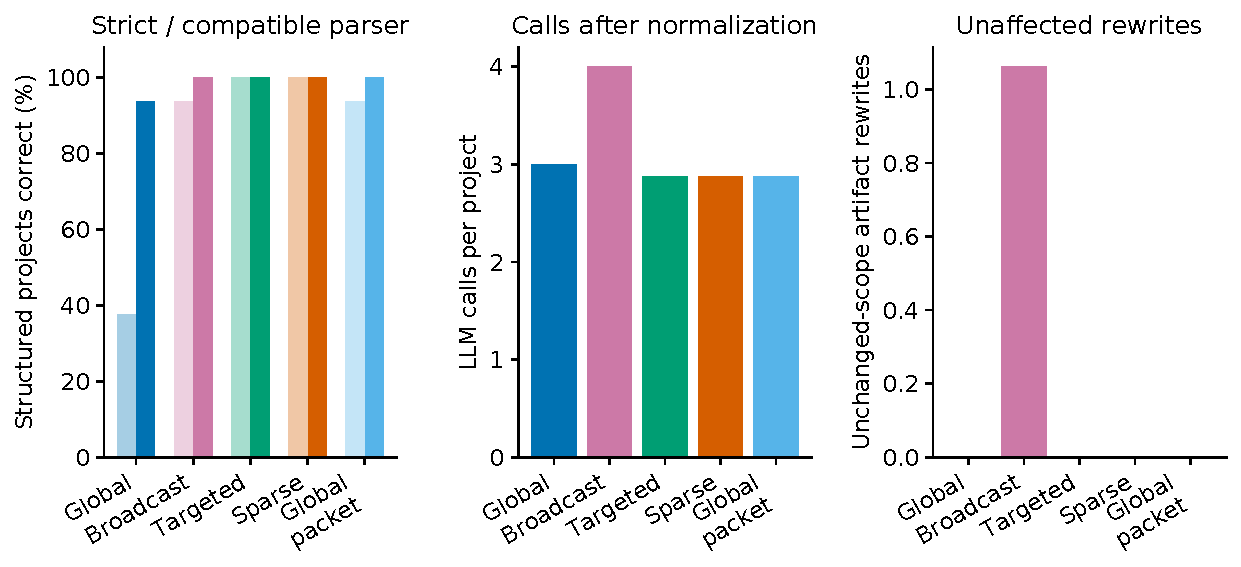
\includegraphics[width=\linewidth]{parser_followup.pdf}
\caption{Post hoc parser sensitivity on the same sixteen inspected replica-0 projects, with fresh GPU continuations. Equivalent explicit tool envelopes are accepted without filling missing task parameters. The original strict-parser results remain visible in faint bars. This is not a new held-out evaluation.}
\end{figure}

\section{Mechanism and limits}
The recipient-selection comparison has a structural limit. For valid original artifacts in this scope-complete graph, changed-contract roles are exactly the roles invalidated by the global check. Both methods then use the same topological order, packet and fallback. The compatible-parser audit confirms identical request sequences, so sampled differences cannot establish a distinctive routing algorithm. A redundant extra inspection in the global implementation is not a fundamental complexity benefit.

In the eight-case exception-corruption stress, completions are 6/8 for global state, 7/8 for broadcast, targeted and sparse, and 8/8 without detailed issue feedback. Targeted and sparse use two rounds; broadcast averages 1.375. This unfavorable control does not support a benefit from more corrective detail. Ordinary-condition broadcast rewrites 35 unaffected artifacts, whereas targeted, sparse and global checking rewrite none. Restoration of a deliberately corrupted appendix is necessary and is not included in that interpretation.

The primary evidence contains 152 groups of repeated identical request payloads. Eleven vary in parsed text and one varies in tool-envelope shape. The April pair has equal normalized tool parameters but different strict-parser acceptance. A May pair instead returns missing arguments versus an explicit usable tool envelope, so one normalized representation still differs. Seeds therefore do not promise bitwise reproduction. In addition, four accepted structured reports for the same project call stock codes customers. The numerical guard does not validate all prose. This directly limits any claim of full report correctness.

The real transactions ground the computations, not the authored workflow or user behavior. Scope and dependencies are registered explicitly. The parameterized pipeline is perfect without LLM calls. We therefore establish a useful execution boundary and an inspectable application, rather than a demonstrated need for multiple LLM agents or measured human attention savings.

\begin{figure}[!htbp]
\centering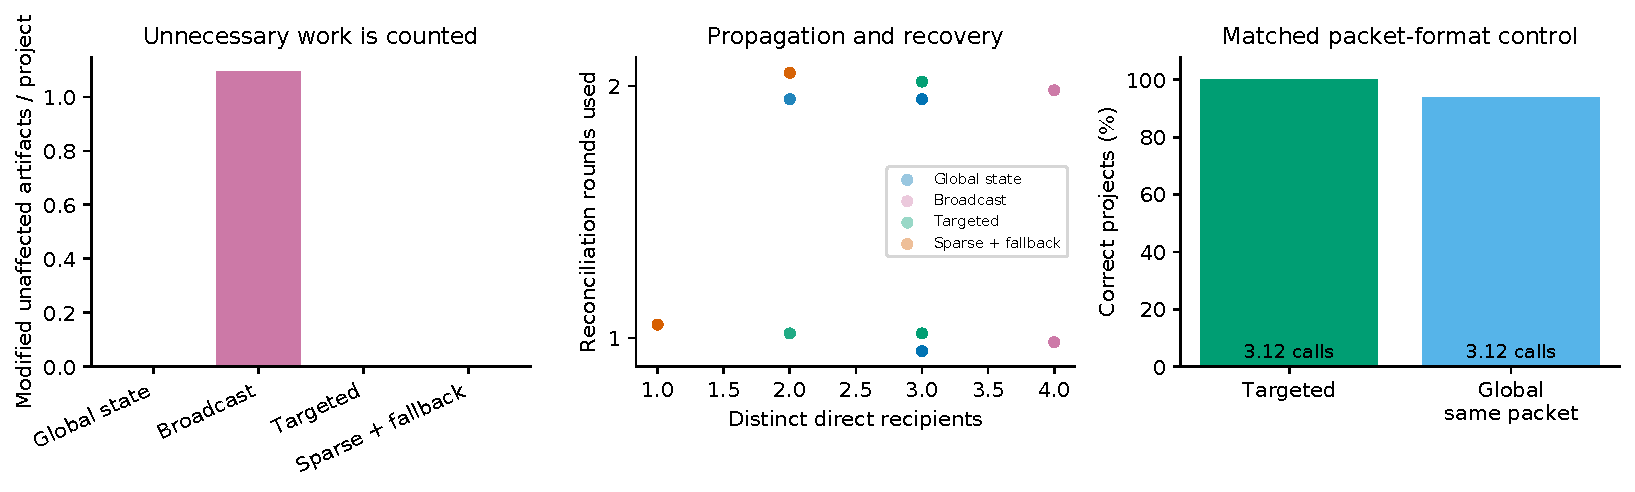
\includegraphics[width=\linewidth]{scope_and_controls.pdf}
\caption{Ordinary strict-parser adaptation on recorded data. Rewrites count artifact identity changes, even when values stay equal. The matched packet-format control uses sixteen replica-0 projects. Recipient count is not independently randomized; the recovery scatter is descriptive.}
\end{figure}
\begin{figure}[!htbp]
\centering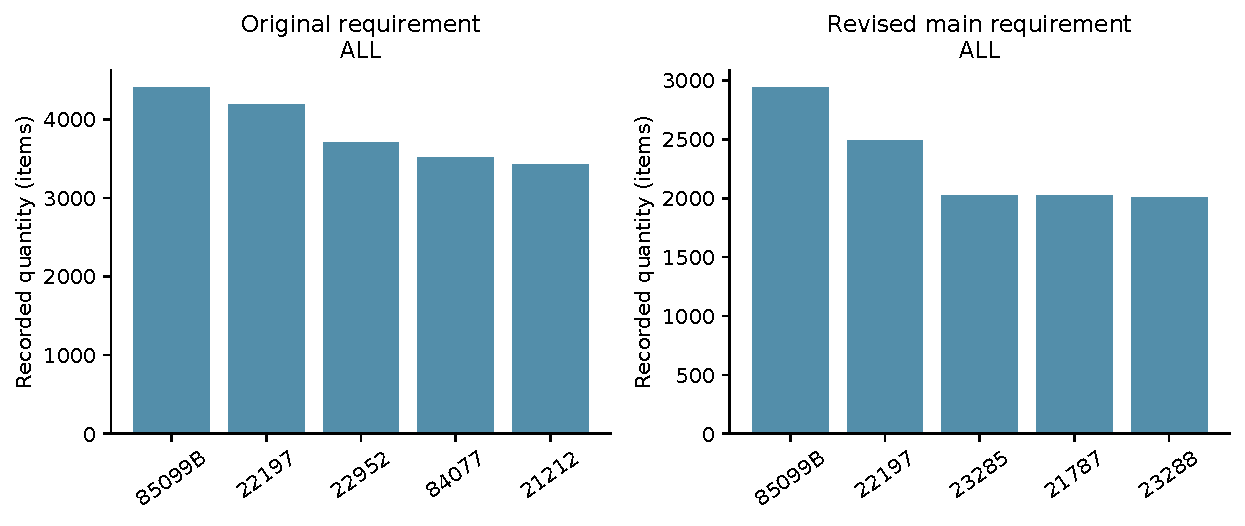
\includegraphics[width=.95\linewidth]{worked_transaction_example.pdf}
\caption{Recorded stock-code aggregates before and after the first qualifying constructed change. The SQL, chart values and numerical report claims are executable; the protected appendix retains the original contract.}
\end{figure}

\section{Relation to prior work}
AIPOM already supports user edits to agent plans, dependency-aware reruns and user-driven repair \citep{kim2025aipom}. InstructFlow uses execution feedback, instruction graphs and symbolic constraints for targeted subgoal correction \citep{chi2025instructflow}. Our contribution cannot be the generic idea of changing a prompt or rerunning dependent agents.

Blackboard systems coordinate analytical work through shared state and specialist help \citep{salemi2026blackboard}. CONSENSAGENT detects debate behaviors and refines prompts to mitigate sycophancy \citep{pitre2025consensagent}. LLM-Flock uses local influence-based plan consensus for robot formations \citep{li2025flock}. Naming-game experiments show that LLM populations can form conventions and collective biases \citep{ashery2025conventions}. These motivate separating agreement from external task correctness.

Event-triggered communication has an established control-theoretic history \citep{nowzari2019event}. Its stability assumptions do not apply automatically to LLM repairs. Incremental build systems already separate scheduling from rebuilding decisions \citep{mokhov2018build}. The present study therefore tests a scoped, executable application protocol against that simpler explanation, rather than claiming a new consensus or scheduling algorithm.

\section{Reproducibility and conclusion}
The separate package preserves the official source checksum, row-level transformation hash, frozen code, prompts, every attempt, source-specific figures and actual response-driven traces. Saved-output reproduction uses no inference. The local Decision desk replays changes and exposes unresolved artifacts. A separate custom-change mode executes the deterministic comparator, clearly labeled as such. Scripted interface checks are not participant data.

Known stage inference comprises 1,316 scheduled requests and 1,315 attempt intents, with 874,657 prompt and 112,851 completion tokens. One interrupted development attempt has unknown returned-token usage; another scheduled request never records a generation intent. The 803 frozen-study calls and 250 exploratory follow-up calls all return successfully. Historical clocks remain intact and no paid resource is provisioned. Final wall-time and shutdown records are in the resource ledger.

For these contracts, the supported choice is the parameterized pipeline or normalized global check. Targeted routing saves active-broadcast notification processing but adds no distinct allocation decision over the matched global control. A useful next investigation is provenance-linked verification of generated narrative claims on new analytical tasks. The observed entity-type error remains unsolved by agreement, version tracking and numerical checks.

\begingroup\small
\bibliographystyle{plainnat}
\bibliography{../../research/coordination_injections/references}
\endgroup
\clearpage
\appendix
\section{Additional empirical and controlled evidence}
\begin{figure}[H]\centering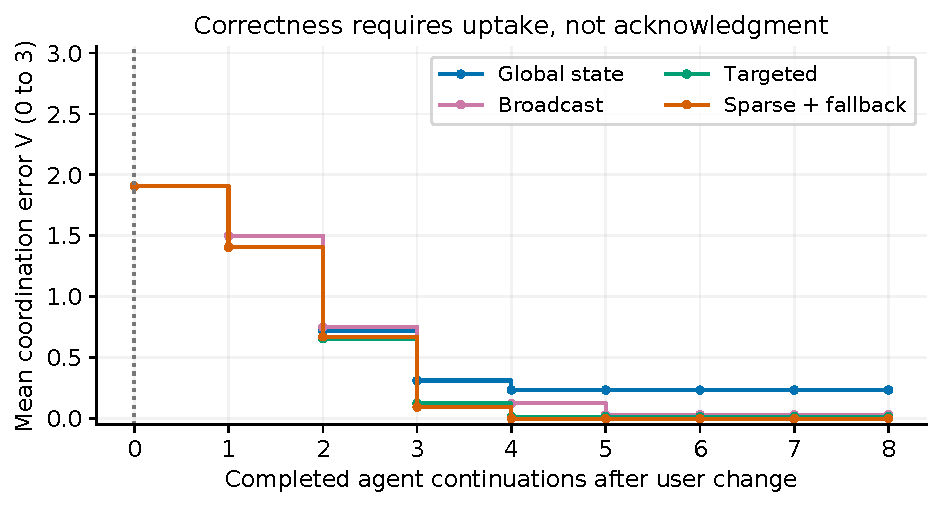
\includegraphics[width=.82\linewidth]{coordination_error.pdf}\caption{Authored coordination error over completed GPU continuations after a change. Stopped runs retain their final values. A declining curve does not establish contraction or isolate intervention value from natural completion.}\end{figure}
\begin{figure}[H]\centering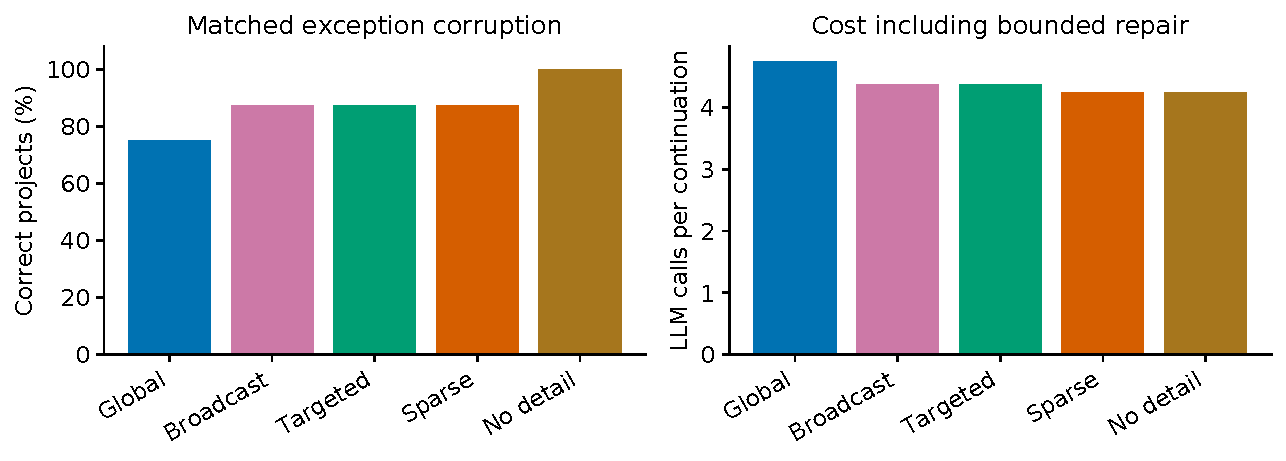
\includegraphics[width=\linewidth]{stress_ablation.pdf}\caption{Separately constructed exception-corruption stress, on eight recorded-data project checkpoints. Every method receives the same corruption. Restoration of an unchanged-contract appendix is necessary repair, not automatically unnecessary work.}\end{figure}
\begin{figure}[H]\centering
\includegraphics[width=\linewidth]{synthetic_boundaries.pdf}\caption{Entirely authored data and controlled responses, zero GPU calls. These cases test mechanisms and failures, not their prevalence.}\end{figure}
\section{Inspecting adaptation}
\begin{figure}[H]\centering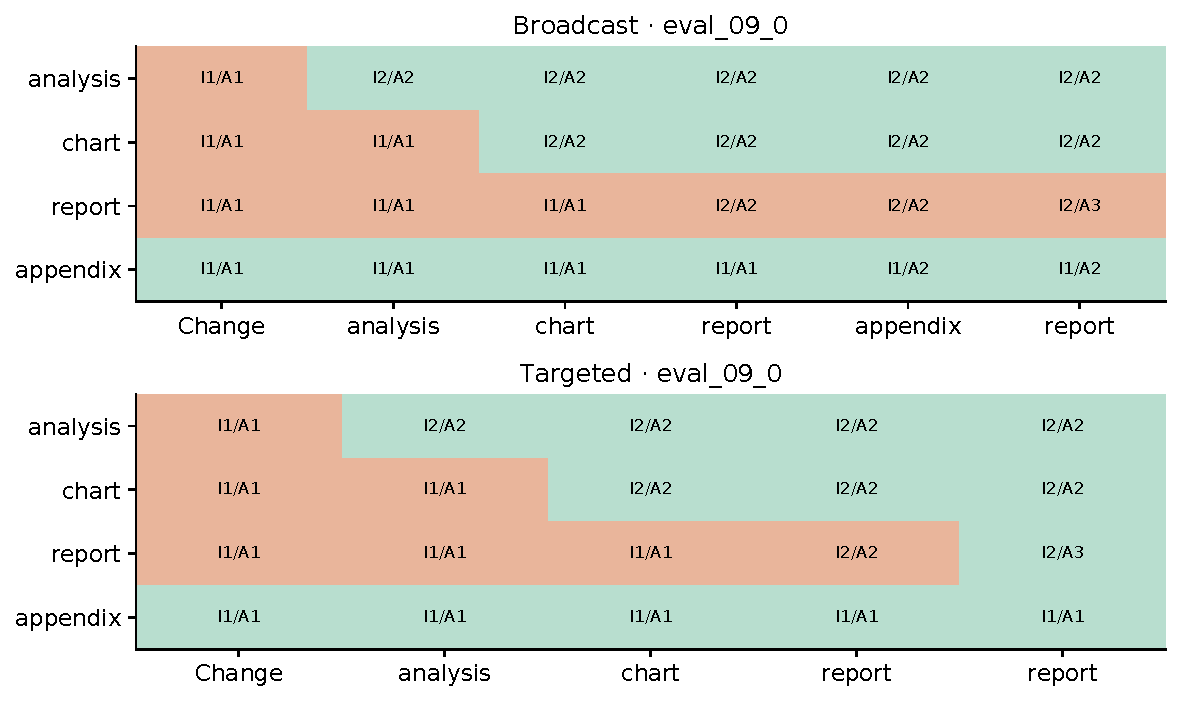
\includegraphics[width=.88\linewidth]{timeline_favorable.pdf}\caption{Favorable strict-parser example selected by the frozen first-ID rule. I denotes consumed contract version and A artifact revision. Green means public checks pass; orange means unfinished. These are recorded GPU/tool events, not human review durations. A tied example is saved separately. No unfavorable replica-0 case qualifies; replica-1 and stress failures remain reported.}\end{figure}

\begin{figure}[H]\centering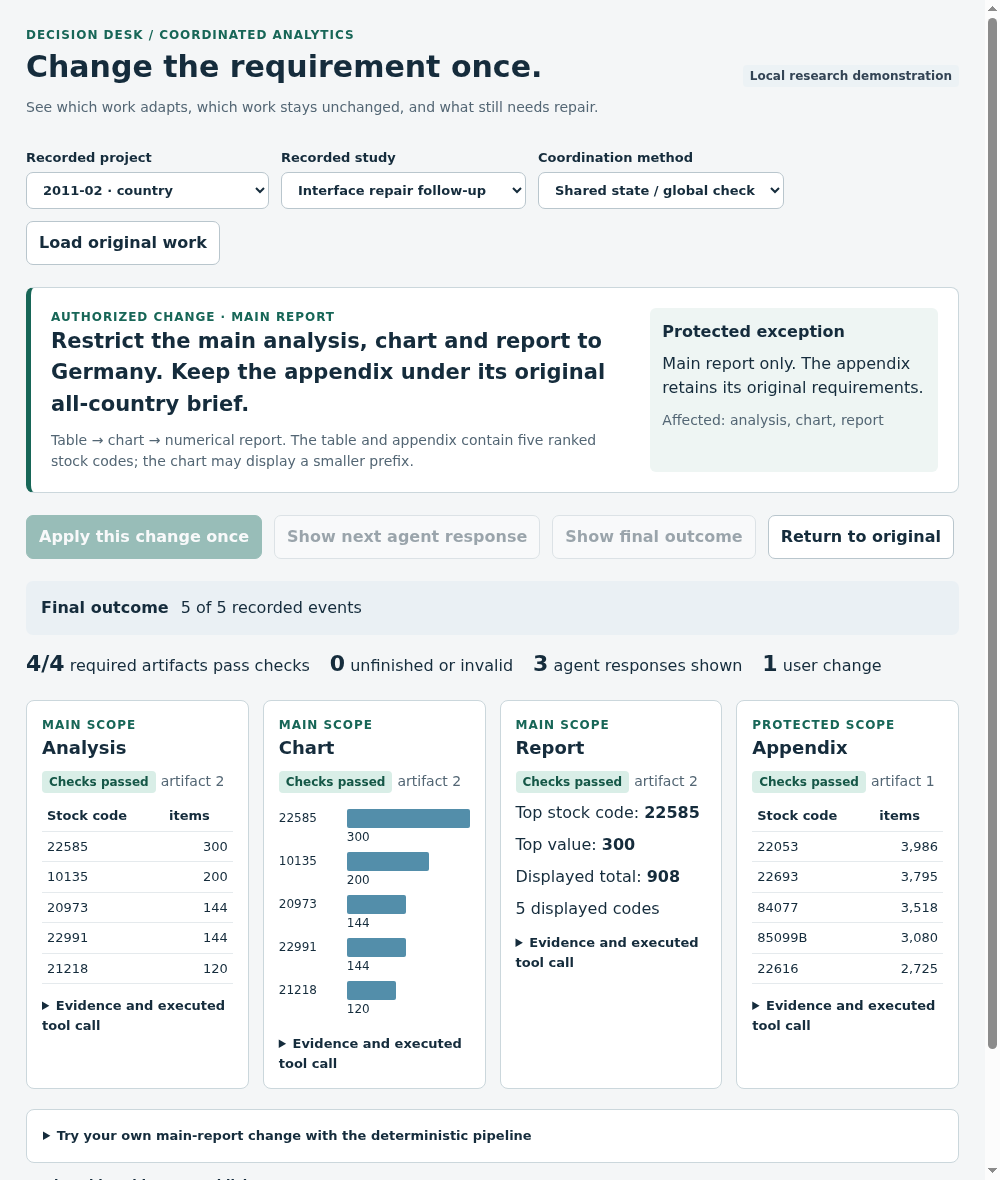
\includegraphics[width=\linewidth]{../../artifacts/coordination_injections/interface_final/compatible_shared_state.png}\caption{Working local interface replaying a real saved GPU continuation from the exploratory interface-repair follow-up. The transactions are recorded; the project and change are authored. Structured checks, affected roles and the protected appendix are visible. The screenshot is a scripted software demonstration, not a user study.}\end{figure}
\end{document}
